% This work by Jeremy A. Hansen is licensed under a Creative Commons 
% Attribution-NonCommercial-ShareAlike 3.0 Unported License, 
% as described at http://creativecommons.org/licenses/by-nc-sa/3.0/legalcode

Problem solving and troubleshooting in programming is often referred to as debugging. 
Does your program not compile? 
Does it not achieve the desired effect? 
Debugging is your answer. 
And, unless you are a perfect programmer, you are likely to do quite a bit of debugging.

The first step to debugging is looking for common errors.

\LevelD{The Compilation Error}

These errors happen when your compiler returns an error message after you hit compile. 
The messages usually tell you what is wrong, and what line the error is on, but be sure to double-check the lines immediately before and after the reported error. 
Because the code is incorrect, the compiler can only guess at what you meant and give you a hint.

\begin{figure}[tbh]
  \centering
  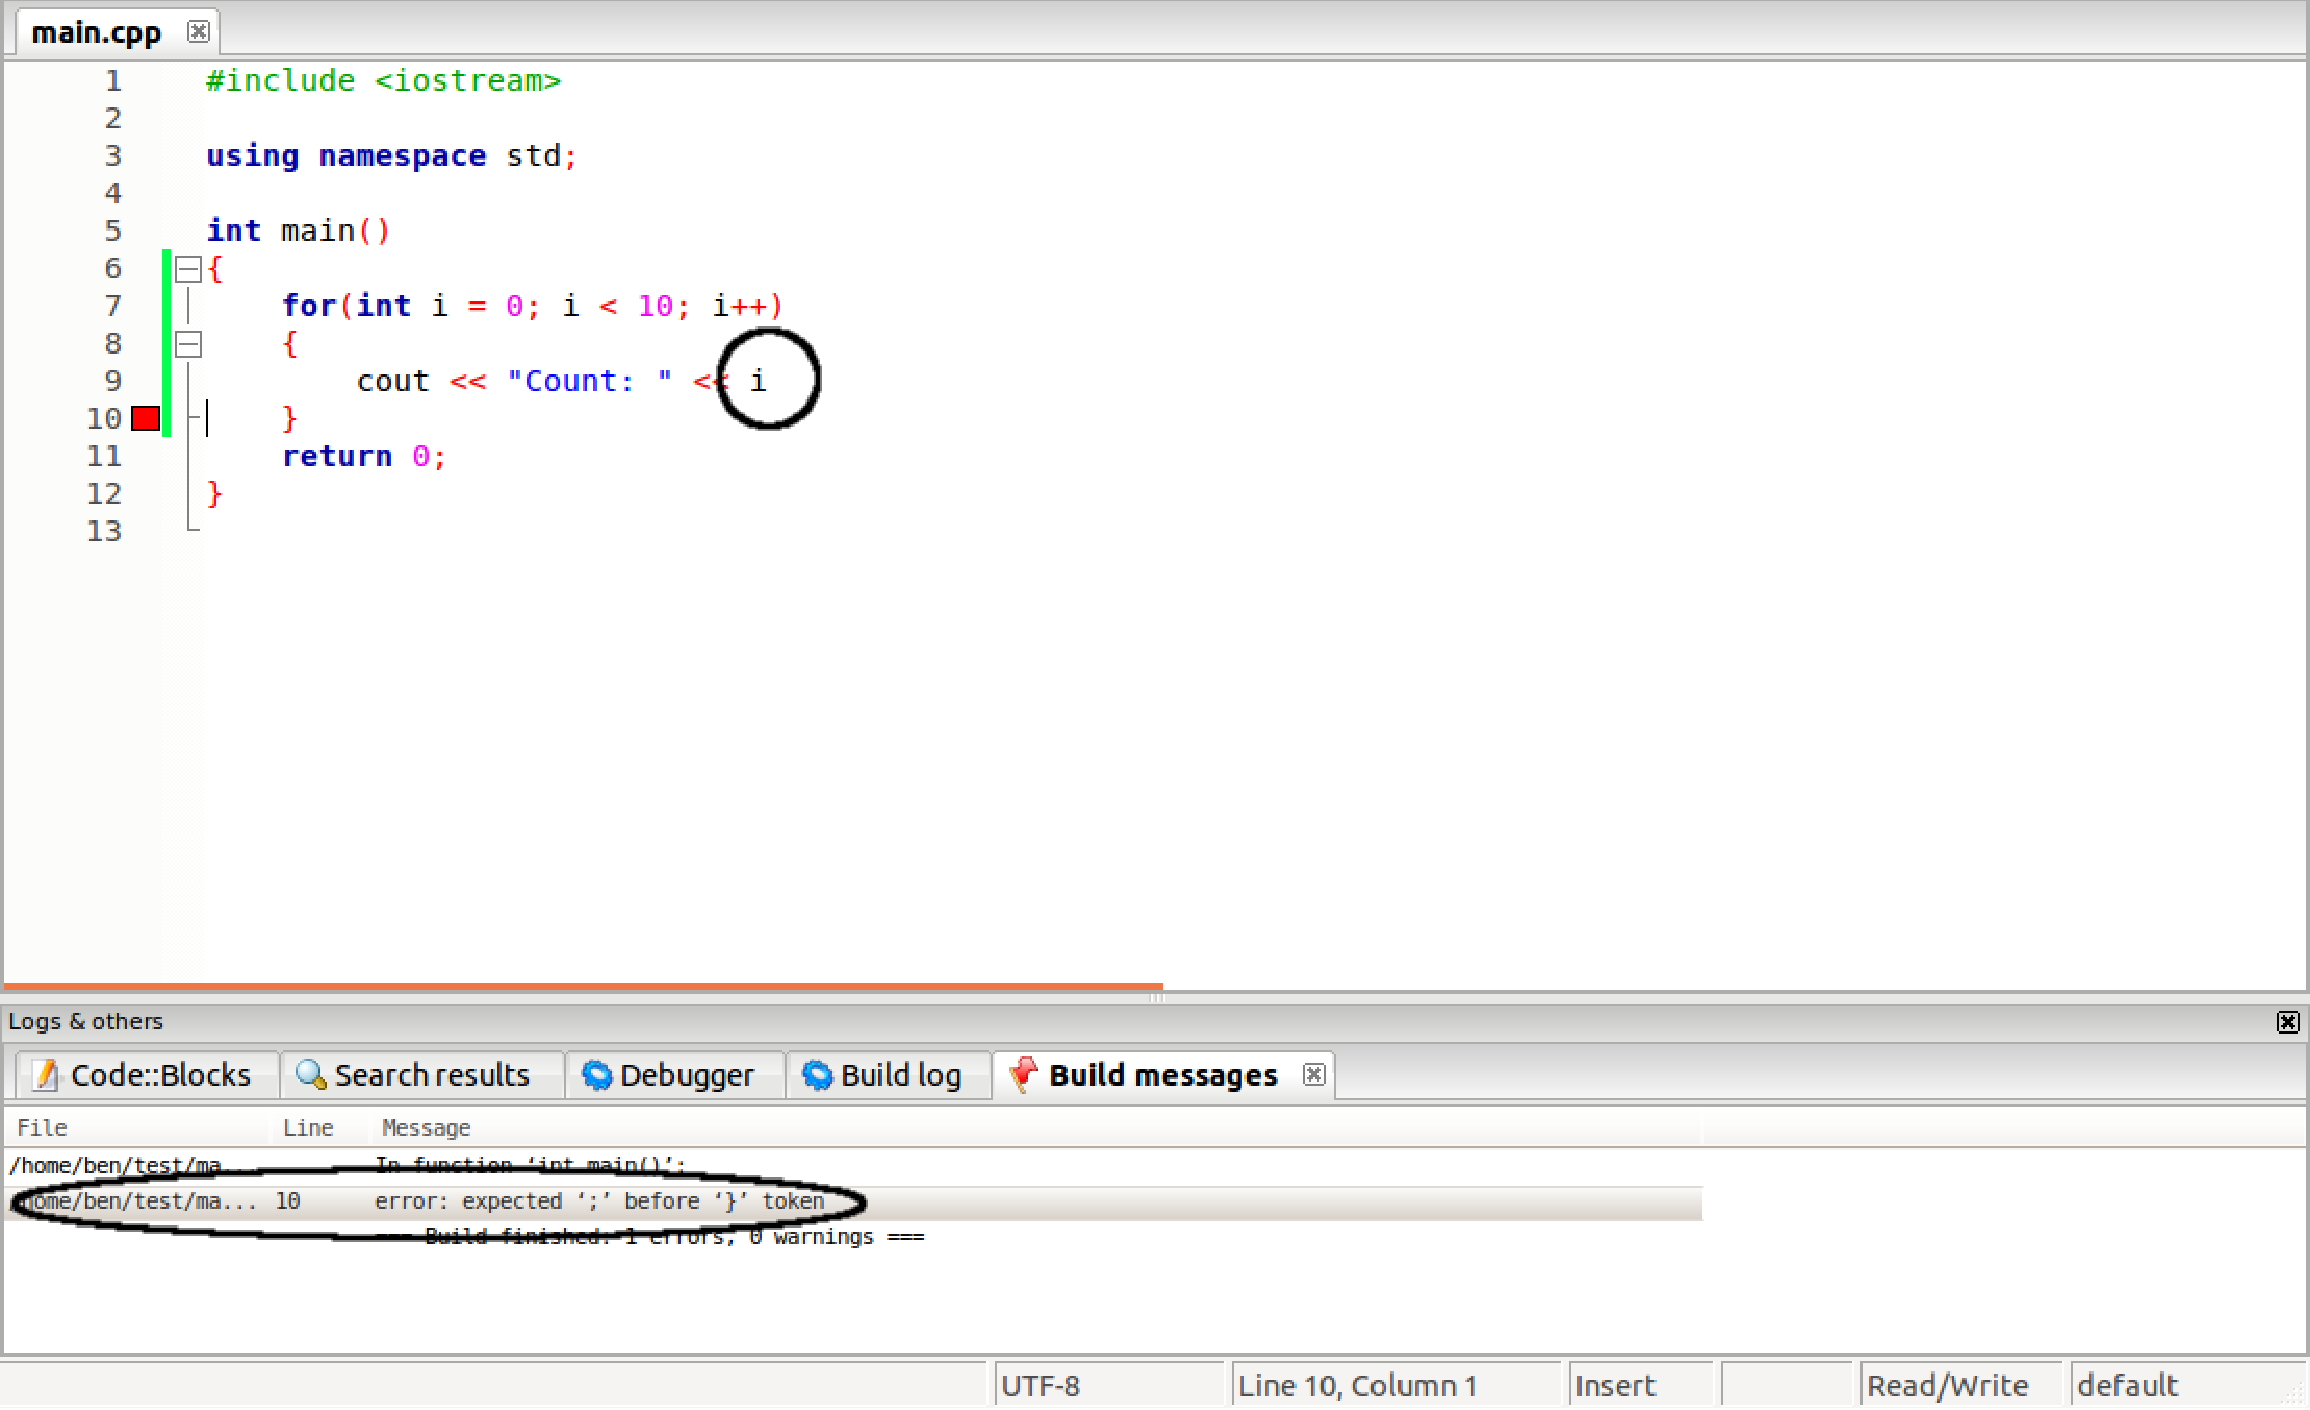
\includegraphics[width=\textwidth]{diagrams/fig-netbeans-syntax-error.pdf}
  \caption{A syntax error in the NetBeans development environment} \label{fig-netbeans-syntax-error} 
\end{figure}

For example, one of the most common errors a beginning programmer will encounter is forgetting a semicolon. 
In some development environments (like NetBeans in Figure \ref{fig-netbeans-syntax-error}), this will cause the error to be reported not on the line with the missing semicolon, but on the following line. 

\LevelD{The Logic Error}

Logic errors are often subtle, and occur after the code compiles. 
When the code is executed, however, the result is wrong. 
This may happen when arithmetic operators like \Code{+}, \Code{-}, \Code{*}, and \Code{/} get mixed up. 
Another common issue is misplacement of parentheses, as a misplaced parenthesis can cause problems in complex expressions. 

\LevelD{The Infinite Loop}

Another specific logic error is the infinite loop. 
The infinite loop is a common error that can result in your program repeating the same block of code over and over. 

For an infinite loop to occur, the conditional expression of a \Code{while}, \Code{for}, or \Code{do-while} loop remains true. 
There are many ways for this to happen, such as accidentally using \Code{=} instead of \Code{==} to compare two numbers, or using the wrong operators, like a \Code{>} in the place of a \Code{<}.

\begin{figure}[tbh]
  \centering
  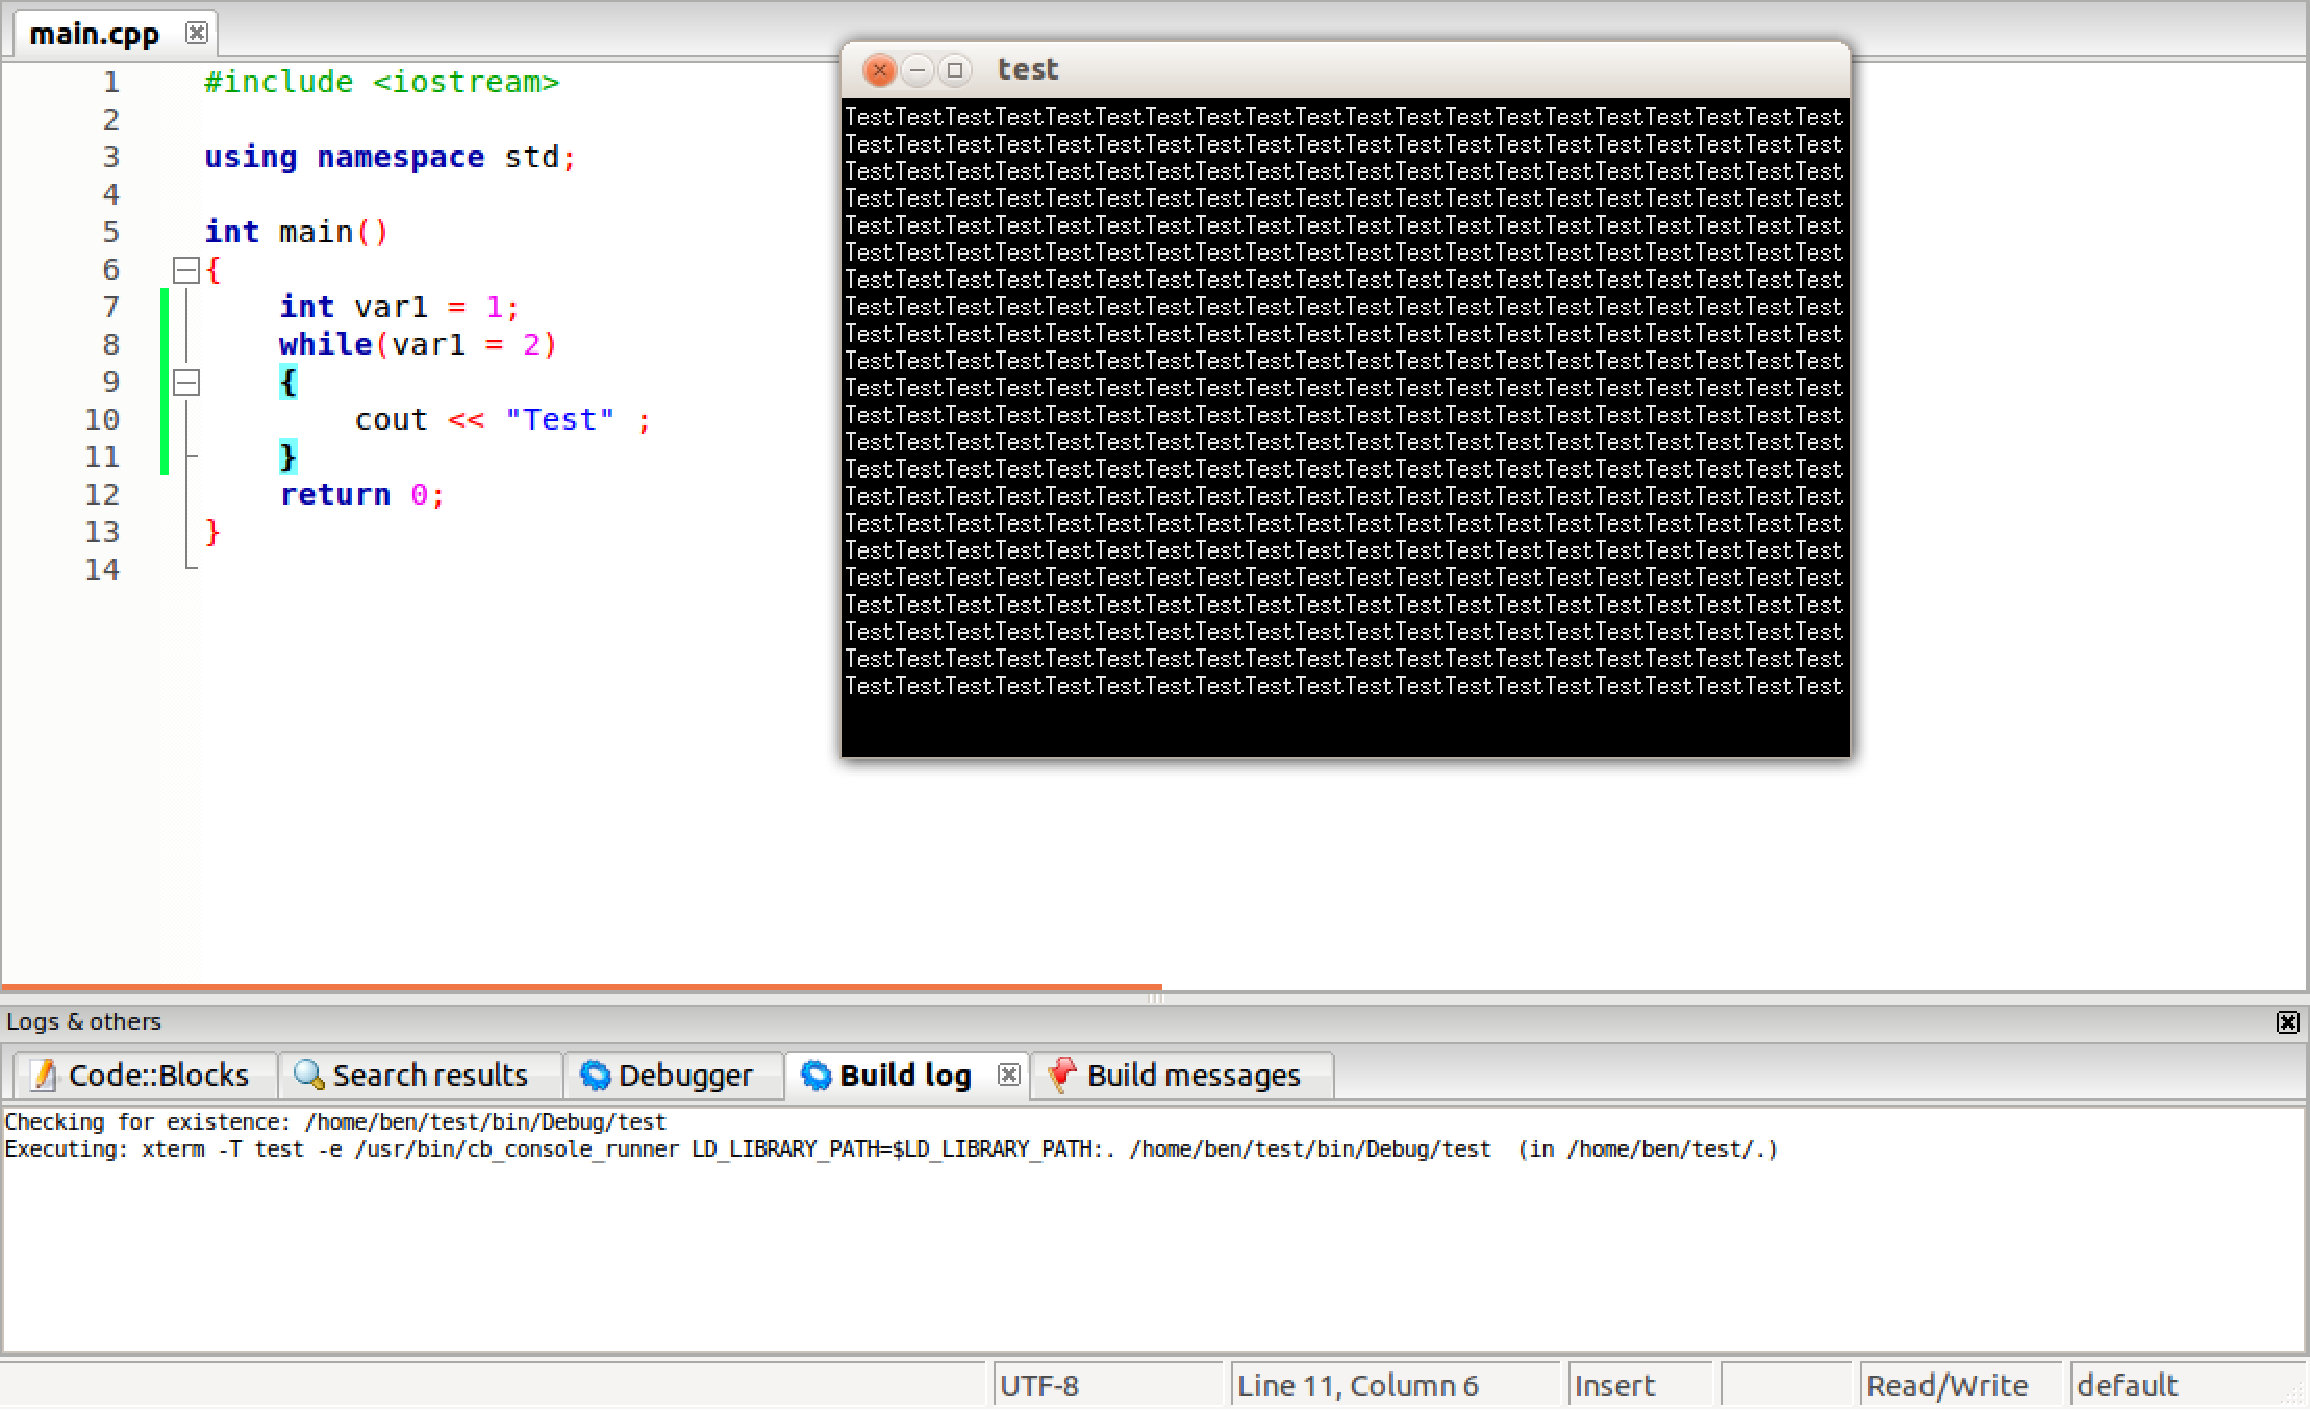
\includegraphics[width=\textwidth]{diagrams/fig-netbeans-infinite-loop.pdf}
  \caption{An infinite loop in the NetBeans development environment} \label{fig-netbeans-infinite-loop} 
\end{figure}


\LevelD{Review Questions}
\begin{enumerate}
	\item Consider the following function:
	
\noindent\begin{minipage}{\linewidth}\begin{lstlisting}
double average (double s1, double s2, double s3, s4);
{
  retun s1+s2+s3+s4/4
}
\end{lstlisting}\end{minipage}

		\begin{enumerate}
		\item Find the syntax errors in the function.
		\item There is a logic error in the function. What is it? How does it affect the output of the code?
		\end{enumerate}

  \item The below program compiles, but does not get the result the programmer wanted. Why?

\noindent\begin{minipage}{\linewidth}\begin{lstlisting}
int main()
{
  int shots, goals, saves;
  double save_perc;
  char cont;

  cout.unsetf(ios::fixed);
  cout.unsetf(ios::showpoint);

  cout << "Enter the number of shots on goal:\t";
  cin >> shots;
  cout << "Enter the number of goals scored:\t";
  cin >> goals;
  cout << endl;

  saves = shots - goals;

  // Hockey shows save % as decimal to three places
  save_perc = (saves / shots); 
  cout << "If there were " << shots << " shots and " 
    << goals << " goals, " 
    << "then the goalie's save percentage was ";

  cout.setf(ios::fixed);
  cout.setf(ios::showpoint);
  cout.precision(3);
  
  cout << save_perc << endl << endl;
  return 0;
}
\end{lstlisting}\end{minipage}


\end{enumerate}

\LevelD{Review Answers}

\LevelD{Further Reading}

\begin{itemize}
\item \url{~}
\item \url{~}
\item \url{~}
\end{itemize}	

